\documentclass[12pt]{article}
\title{Make binary search dynamic}
\author{林橋毅 111502563}
\usepackage[UTF8]{ctex}
\usepackage{graphicx} %插入图片的宏包
\usepackage{float} %设置图片浮动位置的宏包
\usepackage{caption}
\usepackage{subfigure} %插入多图时用子图显示的宏包
\usepackage{algorithm}
\usepackage{cite}
\usepackage{algpseudocode}
\usepackage{amsmath}
\usepackage{graphics}
\usepackage{epsfig}
\usepackage{amssymb}
\usepackage{bm}
\newtheorem{definition}{Definition}

\begin{document}
	\captionsetup[figure]{labelfont={bf}, labelformat={default}, labelsep=period,name={Fig.}}
	
	\maketitle
	
	\part{Introduction}
	本專題的題目是 Make binary search dynamic,顧名思義是讓二分搜尋動態化,可以用對數時間進行搜尋、線性時間插入元素。若結構中有 N 個元素,並且我們可以假設 $N = 2^k$ ,這個結構將會有以下性質:有 $k$ 層,第 $i, 0<=i<k$ 層是一個大小為 $2^i$ 的 array,每層不是空的就是滿的且都是由小到大排序好的。
	\part{Method}
	本節將會介紹我為了這格資料結構所設計的函式。
	\section{resize}
	為了要達成動態大小的資料結構,我設計了 resize 的函式,參考 vector 的方法,每次增加容量都將容量翻倍,這樣可以均攤時間複雜度也可以達到動態調整的功能。
	\begin{algorithm}[H]
		\caption{resize(sizeLayer)}
		\begin{algorithmic}
				
				\State declare new list size = 2*size(old list)
				\State copy the old list to new list 
				\State Assign new list to the structure
				\State Update maxLayer <- sizeLayer
		\end{algorithmic}
	\end{algorithm}
	\section{merge}
		合併是這個資料結構的核心,由 merge 方法為結構中層與層之間提供連結,在插入、刪除都會用到,與 merge sort 的 merge 相似,給定兩層的數據,產生合併後的 array 並且進行 push 的操作,時間複雜度為 $\theta(N)$。
		
		給定 list\_0, list\_1, del\_0, del\_1, layer,合併 list\_0 跟 list\_1 並且放到第 layer + 1 層,其中 del\_0,  del\_1 分別是 list\_0, list\_1 的刪除陣列,如果 list\_k[i]]$k \in \{0,1 \}$ 若被刪除則 del\_k[i] 為 1 反之為 0。
		\begin{algorithm}[H]
			\caption{merge(list\_0, list\_1, del\_0, del\_1, layer)}
			\begin{algorithmic}
				\State Declare new list
				\State declare two pointer p0, p1 <- list\_0.end, list\_1.end
				
				\While{p0 >= 0 and p1 >= 0}
					\If{p0 < 0}
						\State put remain element in list\_1 to new list
					\EndIf
					\If{p1 < 0}
						\State put remain element in list\_0 to new list
					\EndIf
					\If{list\_0[p0] > list\_1[p1]}
						\State put list\_0[p0] to new list
						\State p0-1
					\Else
						\State put list\_1[p1] to new list
						\State p1-1
					\EndIf
				\EndWhile
					
				\If{space is not enough} 
					\State rezise
				\EndIf
				\State update the deletion array 
				\State push new list the next layer
			\end{algorithmic}
		\end{algorithm}
	\section{push}
		為了將合併過後的 array 搬運到下一層,我設計了一個 push 函式,這個 function 檢查下一層是否為空,若為空就可以放到下一層,若不為空就將下層與當前合併過後的 array 進行合併,並且在移動過程中要更新空層的位置,而且還有檢查空間是否足夠進行,若不足就執行 resize 的 function。
		\begin{algorithm}[H]
			\caption{push(n)}
			\begin{algorithmic}
				\If{next layer is empty}
					\State put the layer to next layer
				\Else
					\State merge(this layer, next layer)
				\EndIf
			\end{algorithmic}
		\end{algorithm}
	\section{insert}
		進行插入元素時,給定欲插入的元素 $n$,因為題目要求不能重複插入,所以要檢查是否已存在該元素。插入時,如果第一層是空的就放在第一層,如果不是就跟第一層合併後下推。
		\begin{algorithm}[H]
			\caption{insert(n)}
			\begin{algorithmic}
			\If{n is found in structure}
				\State return Insert Failed
			\EndIf
			\State N++ // N is number of element in the structure
			
			\If{the first layer is empty}
				\State Input n the the first layer
			\ElsIf{the first layer is full}
				merge(n, first layer ,0) // 0-th layer
			\EndIf
			\State return Insert Success 
			\end{algorithmic}
		\end{algorithm}
		
	\section{find}
	搜尋指令是指在給定目標值,搜尋該值在資料結構中的位置。由於每一層的 array 都是排序好的,所以我們可以依續使用二分搜尋每一層是否存在想要查詢的值,就可以快速建構查詢指令。理論上,二分搜尋法的時間複雜度是 $\theta(N)$ N 是欲搜尋陣列的元素數量。假設我們有 $M$ 個元素,總共有 $lg(M)$ 層 array,且第 $i$ 層的 array 元素數量為 $2^i, i >=0$,我們可以推測搜尋的時間複雜度為 $\theta((lgM)^2)$
	\begin{algorithm}[H]
	\caption{find(n, layer)}
	\begin{algorithmic}
			\If{layer > base} 
				\State return -1
			\EndIf
			\State binary search for n in layer-th layer
			\If{found n in layer-th}
				\State return found
			\ElsIf{not found}
				\State return find(n, layer+1)
			\EndIf
	\end{algorithmic}
\end{algorithm}
	\section{delete}
	進行刪除操作時,先搜尋到該元素,刪除後得要整理我們的結構以騰出空間,不過不必過於積極整理結構,可以使用一個表格紀錄該元素是否已經被刪除,如果查詢到已被刪除的元素就可以直接回答刪除,刪除時順便檢查該層已被刪除的元素數量是否為該層應有元素的一半,若有就可以跟上一層合併。
	\begin{algorithm}[H]
		\caption{delete(n)}
		\begin{algorithmic}
			\If{n is not existed}
				\State return Delete Failed
			\EndIf
			
			\State Delete element by record a array
			
			\If{number of element are deleted this layer == half of size of this layer}
				\State declare new list called tidyList
				\State iterate the old list and add element which didn't deleted to tidyList
				\If{previous layer is full}
					\State merge(previous layer, tidyList)				
				\Else
					\State put the tidyList the previous layer
				\EndIf
			\EndIf
			
		\end{algorithmic}
	\end{algorithm}
	\part{Experiment}
		為了實測這個資料的資料結構並且與紅黑樹相比較,我設計一個簡單的測驗:給定數字 $N$,進行 $N$ 次測試,第 $i, \ (0<=i<=N)$ 次測試分別測試插入 $1$ 到 $i$、查詢 $1$ 到 $i$、刪除 $1$ 到 $i$,接著個別紀錄插入、查詢、刪除的時間。
		
		可以發現無論是插入、查詢、刪除都的時間表現都比紅黑樹要差,插入時間與紅黑樹非常接近,但在查詢跟刪除與紅黑樹差距較大,與理論上較符合。
		
		\begin{figure}[H]
			\centering
			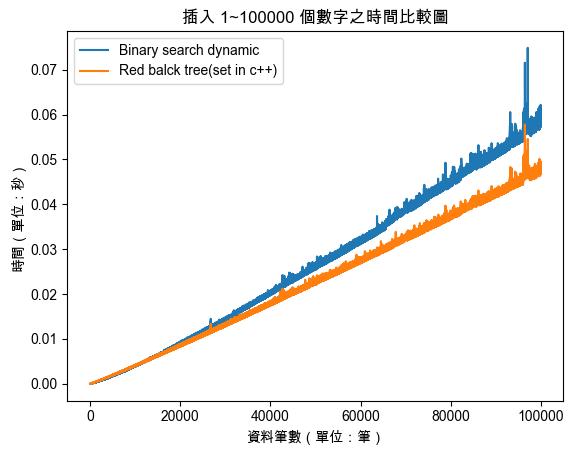
\includegraphics[width=0.7\textwidth]{insert.png}
			\caption{插入時間比較圖} %最终文档中希望显示的图片标题
			\label{Fig.main1} %用于文内引用的标签
		\end{figure}
		
		\begin{figure}[H]
			\centering
			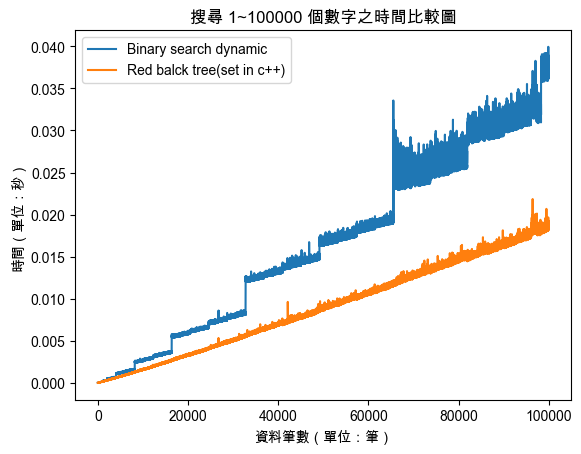
\includegraphics[width=0.7\textwidth]{search.png}
			\caption{搜尋時間比較圖} %最终文档中希望显示的图片标题
			\label{Fig.main2} %用于文内引用的标签
		\end{figure}
		\begin{figure}[H]
			\centering
			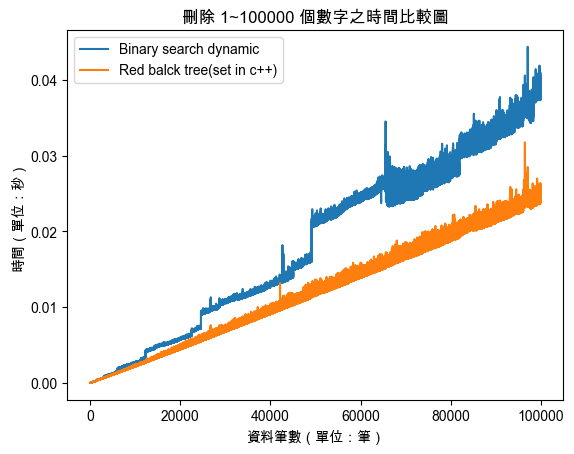
\includegraphics[width=0.7\textwidth]{delete.png}
			\caption{刪除時間比較圖} %最终文档中希望显示的图片标题
			\label{Fig.main3} %用于文内引用的标签
		\end{figure}
	\part{Conclusion \& Reflection}
		本篇實作了動態二分搜尋,是一個相較於紅黑樹更直觀且複雜度也表現良好的資料結構,在易寫性及複雜度上取得相當好的平衡,在插入元素時與紅黑樹表現相當,但在搜尋跟刪除略輸一些,但在刪除時的空間壓縮仍需要在未來將其完善。\\
		
		在這次專題中,我更深入接觸記憶體的操作及管理,雖然在撰寫方面仍有許多不熟練,但已進步許多也讓我知道如何設計一個資料結構跟分解需要使用的方法,這次我就先實作出 merge 的方法後圍繞著 merge 將 insert push 撰寫完成,讓我有設計程式結構的經驗。不過我認為我在細節部分仍要加強,感覺可以在將程式更精簡及加速。

\end{document}